\chapter{Exécution pratique du CAS}

\begin{center}
    \makebox[\textwidth]{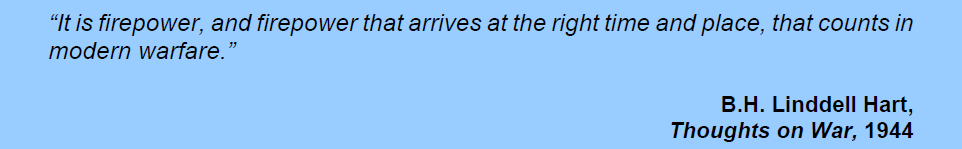
\includegraphics[width=\paperwidth]{quote5.png}}
\end{center}

\section{Introduction}

L'exécution du \gls{cas} commence lorsque la cible est désignée par le \gls{gc} soutenu, et décrit les considérations à prendre en compte pour intégrer le \gls{cas} aux manoeuvres de l'unité soutenue.

\section{Engagement de la cible lors du CAS}

Cette section décrit les procédures tandard lors du \gls{cas}. Bien que certaines opérations nécessitent des procédures spécifiques, le personnel impliqué dans le \gls{cas} doit être familier avec le format standard.

\e
    \item Création du briefing par le \gls{jtac}\\ \\
    Lorsqu'une cible a été déisgnée par le \gls{gc}, le \gls{jtac} doit effectuer les tâches suivantes:
    \ee
        \item Réassembler les informations à propos de la cible
        \eee
            \item Elevation de la cible (ligne 4)\\ \\
            Par défaut, l'élévation est exprimée en pieds au dessus de la mer (ft \gls{msl})
            \item Description de la cible (ligne 5)\\ \\
            La description de la cible doit être concice et précise (par ex. ``5 chars dans un champ''). Le \gls{jtac}/\gls{faca} doit éviter d'utiliser des descriptions compliquées ou des termes qui risquent de ne pas être compris par les pilotes. Cependant, la descrition doit rester spécifique. si le \gls{gc} veut attaquer une \gls{hvt} qui se trouve dans un building à deux étages, il devra spécifier "\gls{hvt} dans building à 2 étages", et pas seulement "building à 2 étages".
            \item Position de la cible (ligne 6)\\ \\
            Le \gls{jtac}/\gls{faca} doit évaluer la précision minimale nécéssaire pour les coordonnées de la cible pour accomplir les objectifs du \gls{gc}. Un largage de bombe guidée laser depuis un émetteur au sol demandera des coordonnées beaucoup moins précises qu'une largage de \gls{jdam}.
                \eeee
                    \item Association du terrain et d'une carte\\ \\
                    Le moins précis, mais rapide et efficace en fonction de la situation.
                    \item \gls{lrf} couplé au \gls{gps} et/ou la boussole\\ \\
                    Sujet à l'imprécision de la boussole, et au brouillage \gls{gps}. Si le brouillage \gls{gps} est possible, une autre méthode devra être utilisée.
                    \item Logiciel de ciblage
                    \item Coordonnées dérivées des images de reconnaissance
                \ed
            \item Positions alliées (ligne 8)\\ \\
            La positions des unités alliées au sol sont données à partir de la position de la cible. La direction est donnée de manière cardinale ou sous-cardinale, et la distance est exprimée en mètres. L'observateur ou le \gls{jtac} peuvent ne pas être l'unité alliée la plus proche de la cible.
            \item Effet souhaité par le \gls{gc}\\ \\
            L'effet souhaité par le \gls{gc} est déterminé en parlant avec lui. Le \gls{jtac} doit offrir au \gls{gc} une estimation réaliste des possibilités en fonction des appareils disponibles, de l'armement embarqué, et de son expertise.
        \ed
    \ed
    \item Requête de \gls{cas}
    \ee
        \item Une fois que la position de la cible a été grossièrement estimée, le \gls{jtac} doit envoyer la demande de \gls{cas} le plus vite possible, pour prendre en compte le temps nécessaire avant l'arrivée des appareils. Il ne fautpas retarder l'envoi de la demande pour augmenter la précision des coordonnées de la cible. \important{Il ne faut jamais utiliser les coordonnées des unités alliaées comme coordonnées cible dans une demande de \gls{cas}.}
        \item Création du game plan\\ \\
        Au minimum, le game plan contiendra le type de contrôle et la méthode d'attaque. D'autres informations peuvent être intégrée au game plan ou être ajouté plus tard aux remarques du CAS brief: les intentions du \gls{gc}, l'effet désiré, l'intervalle entre les appareils dans le cas d'une attaque simultanée par plusieurs éléments \gls{cas}. Dans le cas d'attaques séquentielles (\gls{sead}, marquage), une attention particulière devra être apportée à l'établissement de la séparation entre les appareils. L'objectif du \gls{jtac} n'est pas de dicter aux appareils de \gls{cas} les tactiques à employer, mais de fournir un plan qui correspond aux intentions du \gls{gc}.\\ \\
            Voici un déroulement logique lors de l'établissement du game plan:
            \eee
                \item Déterminer l'effect désiré\\ \\
                La première chose à faire consiste à déterminer l'effet souhaité. Pour cela, il faut prendre en compte:
                \eeee
                    \item Composition de la cible (blindage)
                    \item Répartition de la cible (centré sur un point ou dispersé)
                    \item Position (dégagée ou protégée)
                    \item Dégâts collatéraux potentiels
                    \item Proximité des unités alliées
                \ed
                \item Choisir le type de \gls{tac}\\ \\
                Le type de \gls{tac} dépend de l'armement employé, de la manière manière de réduire les risques, de la vitesse de l'engagement et dela capacité du \gls{jtac} à voir la cible et/ou l'appareil qui attaque.
            \ed
    \ed
\ed

\e
    \item Déroulement d'une mission \gls{cas}:
    \begin{figure}[H]
        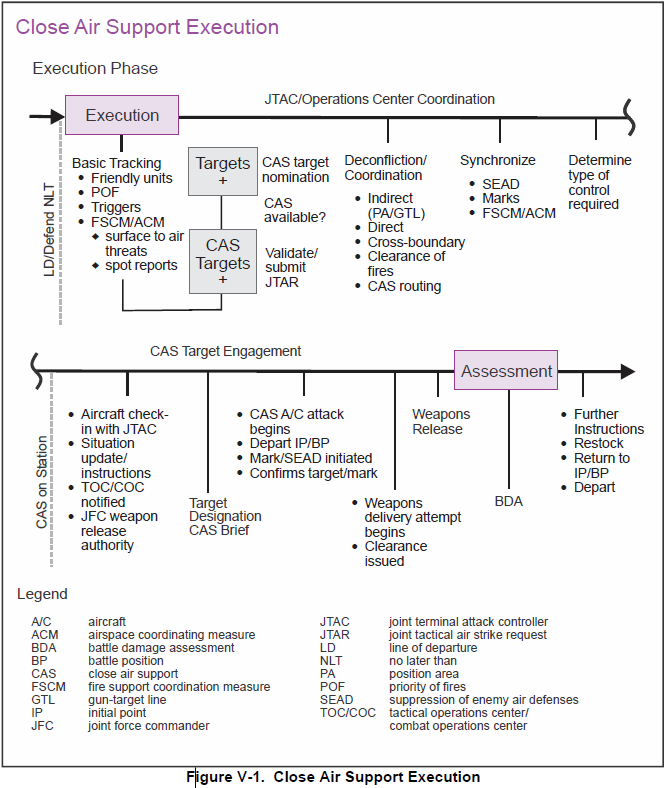
\includegraphics[width=\textwidth]{execution-full.png}
        \caption{Déroulement d'une mission.}
        \label{fig:casflow-full}
    \end{figure}
    \item Cas flow simplifié:
    \begin{figure}[H]
        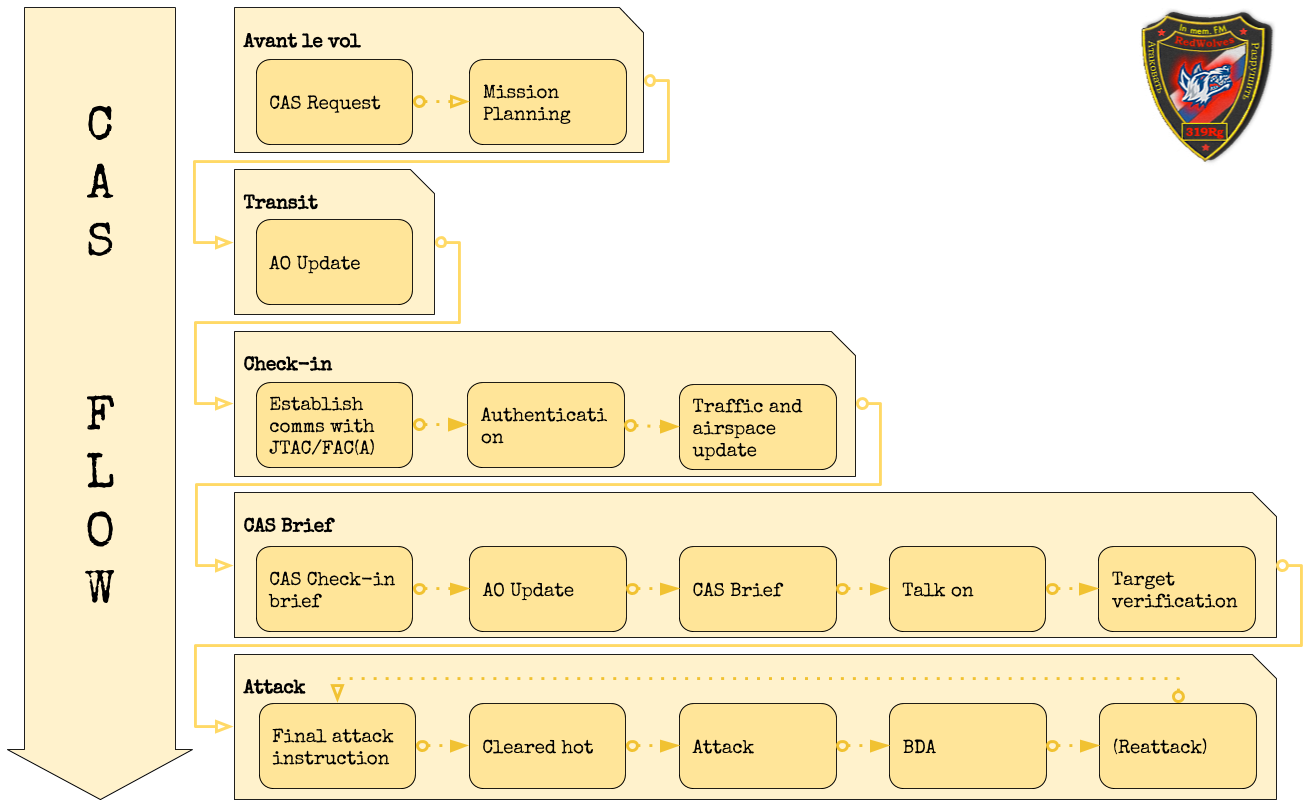
\includegraphics[width=\textwidth]{CASFlow.png}
        \caption{Cas flow simplifié.}
        \label{fig:casflow}
    \end{figure}
\ed

\e
    \item
    Ce chapitre présente le déroulement pratique d’une mission \acrshort{cas}. Le template qui y est présenté illustre une mission \acrshort{cas} typique, et fournit un guide pour le \acrshort{jtac}/\acrshort{faca} et le pilote pour les aider à remplir leur mission.
    \item Le déroulement présenté ici commence après le décollage, et se termine lorsque la patrouille de \acrshort{cas} est sur le retour.
\ed

\section{Routing}
\e
    \item Le routing consiste à diriger les appareils d’un point à un autre.
    \item Extrait du \jp:\\
    \begin{figure}[H]
        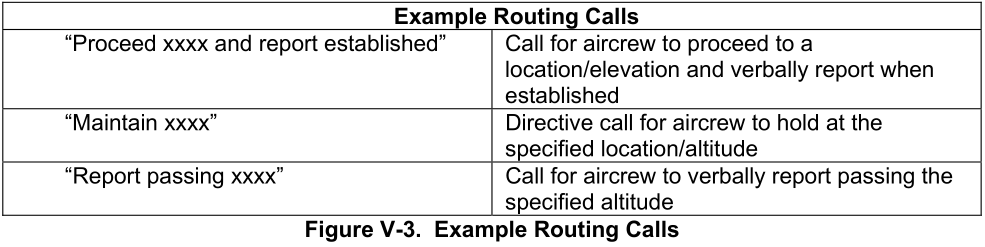
\includegraphics[width=\textwidth]{routing.png}
        \caption{Routing.}
        \label{fig:routing}
    \end{figure}
    \item Exemples:\\
    \ee
        \item Routing standard, demande de maintien de position:\\
        \begin{figure}[H]
            
\includegraphics[width=\textwidth]{routing_ex1.png}
            \caption{Routing: maintien de position.}
            \label{fig:routingpos}
        \end{figure}
        \item Si le contrôleur n'est pas certain de la position et de l'altitude de l'appareil, il doit demander les informations:\\
        \begin{figure}[H]
            
\includegraphics[width=\textwidth]{routing_ex2.png}
            \caption{Routing: demande d'information.}
            \label{fig:routinginfo}
        \end{figure}
        \item Ordre de se diriger vers un point:\\
        \begin{figure}[H]
            
\includegraphics[width=\textwidth]{routing_ex3.png}
            \caption{Routing: ordre.}
            \label{fig:routingorder}
        \end{figure}
        \item Information relative à une menace:\\
        \begin{figure}[H]
            
\includegraphics[width=\textwidth]{routing_ex4.png}
            \caption{Routing: information menace.}
            \label{fig:routingthreat}
        \end{figure}
        \item Information relative aux activités alliées:\\
        \begin{figure}[H]
            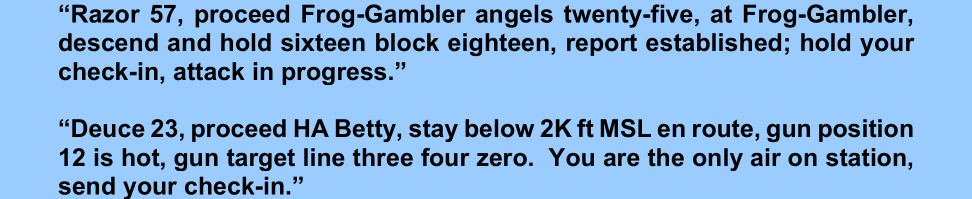
\includegraphics[width=\textwidth]{routing_ex5.png}
            \caption{Routing: information alliés.}
            \label{fig:routingallies}
        \end{figure}
    \ed
\ed

\section{Check-in}

\e
	\begin{minipage}{\linewidth}
    \item
    Le check-in est la première phase du \acrshort{cas} en tant que tel. C’est l’appel effectué de l’appareil en \acrshort{cas} vers le \acrshort{jtac}/\acrshort{faca} pour lui signifier qu’il est prêt à remplir sa mission de \acrshort{cas}.
    \item Comme le check-in peut prendre un certain temps, un appel préliminaire devrait être effectué. Par exemple:
	\begin{lstlisting}[caption=Appel préliminaire, label=preliminary_call]
    PIRATE, ici REDWOLF, pour check-in, quand dispo.
	\end{lstlisting}
	\end{minipage}

	\begin{minipage}{\linewidth}
    \item Format du check-in:
    \begin{figure}[H]
        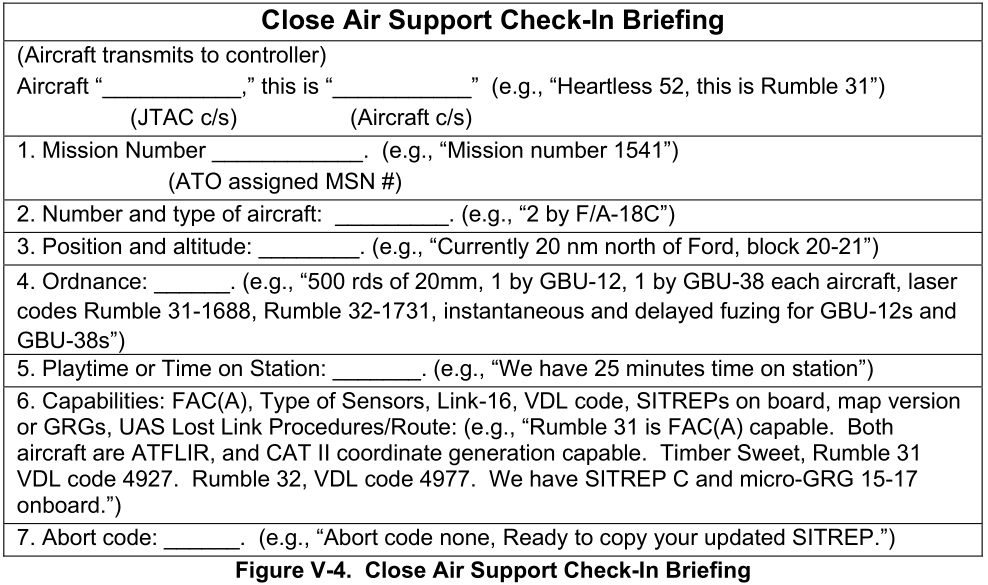
\includegraphics[width=\textwidth]{checkin.png}
        \caption{Format check-in.}
        \label{fig:checkin}
    \end{figure}    
    \end{minipage}
    
    \begin{minipage}{\linewidth}
    \item S'il le souhaite, le \gls{jtac}/\gls{faca} peut demander un check-in abrégé:
    \begin{figure}[H]
        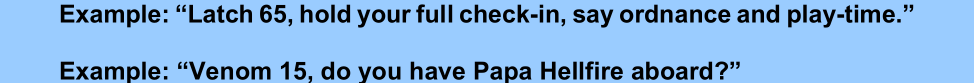
\includegraphics[width=\textwidth]{abbregcheckin.png}
        \caption{Format check-in abrégé.}
        \label{fig:abbregcheckin}
    \end{figure}
    \end{minipage}
    
    \item Le code d’annulation (ligne 7) est un code alphabétique servant à authentifier la directive “Abort” du J-TAC/FAC(A).
    
    \begin{minipage}{\linewidth}
    \item Exemple de check-in:
    \begin{lstlisting}[caption=Check-in, label=checkin]
	PIRATE ici REDWOLF
    	Mission 1234
	    2 Kamov
	    20km au sud de Poti, 500m MSL
    	24 Vikhrs, 80 roquettes, full guns
	    Playtime 30 minutes
    	Senseurs: Shkval
	    Abort code: X-RAY TANGO ZULU
	\end{lstlisting}
    \end{minipage}
\ed
